\section{Problem Definition}
\label{sec:problem_def}
Transactions in traditional database systems satisfy the four ACID  properties: Atomicity, Consistency, Isolation, and Durability. ACID transactions guarantee leaving the database in a consistent state. However, in a web service environment ACID properties and transactional concurrency cannot be fulfilled, due to performance issues. Common occurrences in web service environments involve the collaboration of multiple web services to fulfill a particular task without coupling all the needed operations in one service. Languages, such as BPEL (Business Process Execution Language) \cite{BPEL}, allow a large majority of these business processes to execute web services that must access the underlying database management systems (DBMS). These transactions may be required to relax the isolation property of the database in order to accommodate concurrent transactions.

In the event that a transaction fails (abort), and there are transactions depending on the successful execution of the failed transaction, a cascading rollback must occur, due to the inconsistency of the database. This occurs often in the web service environment due to the relaxed atomicity and isolation properties. The relaxation of the atomicity property allows operations within a transaction to commit any changes performed by the operation permanently before the entire transaction has been completed. The relaxation of the isolation property allows the interleaved execution of operations on a particular resource from concurrent transactions. This improves performance tremendously; however, in the event an operation fails, causing an abort to be issued, every transaction depending upon the failed operation must be aborted as well in order to restore consistency. These compensation transactions have become a standard practice in web service environments but sacrifice the consistency of the system. The next section will discuss a use-case scenario where this problem exists.

\subsection{Use-Case Scenario}
\label{subsec:use_case}
Assume that an e-commerce web site allows users to purchase products through an online interface. When a customer places an order a ticket is generated (see Figure \ref{fig:e_com_ticket}) containing information about the user and purchase. The ticket from the site is then handed off to a business process (starting at $WS_{1}$ in Figure \ref{fig:bp_env}) containing multiple web services, on multiple databases in a distributed context. Figure \ref{fig:bp_env} displays the architecture of the back-end business process in sequence.

\begin{figure}[h]
\captionsetup{justification=centering}
\centering % used for centering Figure

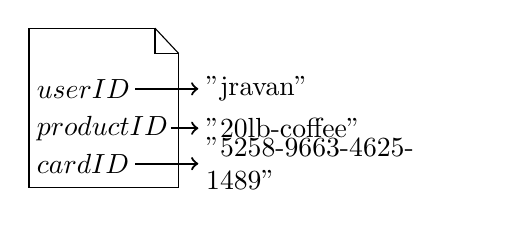
\begin{tikzpicture}
  \draw (0,0) -- (0,2.02) -- (1.6,2.02) -- (1.6,1.7) -- (1.9,1.7) -- (1.9,0) -- cycle;
  \draw (1.6,2.02) -- (1.9,1.7);
  \node[text width=1.5cm] at (.85,1.25) {$userID$};
  \node[text width=1.5cm] at (.85,.75) {$productID$};
  \node[text width=1.5cm] at (.85,.3) {$cardID$};
  \draw[thick,->] (1.35,1.25) -- (2.15,1.25);
  \draw[thick,->] (1.8,.75) -- (2.15,.75);
  \draw[thick,->] (1.35,.3) -- (2.15,.3);
  \node[text width=3.5cm] at (4,1.25) {"jravan"};
  \node[text width=3.5cm] at (4,.75) {"20lb-coffee"};
  \node[text width=3.5cm] at (4,.3) {"5258-9663-4625-1489"};
\end{tikzpicture}

\caption{e-Commerce Web Site Ticket Example} % title of the Figure
\label{fig:e_com_ticket} %% label to refer figure in text

\end{figure}

\begin{figure}[h]
\captionsetup{justification=centering}
\centering % used for centering Figure

\begin{tikzpicture}
    \node [webservice, anchor=north] (ws4) {$WS_{4}$};
    \node [webservice, above=2cm of ws4.north, anchor=north] (ws3) {$WS_{3}$};
    \node [webservice, above=2cm of ws3.north, anchor=north] (ws2) {$WS_{2}$};
    \node [webservice, above=2cm of ws2.north, anchor=north] (ws1) {$WS_{1}$};
    \node [draw, cylinder, shape border rotate=90, aspect=0.75, %
      minimum height=30, minimum width=30, anchor=north, left=.5cm of ws3] (data3) {DB};
    \node [draw, cylinder, shape border rotate=90, aspect=0.75, %
      minimum height=30, minimum width=30, above=2cm of data3.north, anchor=north] (data2) {DB};
    \node [draw, cylinder, shape border rotate=90, aspect=0.75, %
      minimum height=30, minimum width=30, above=2cm of data2.north, anchor=north] (data1) {DB};
    \node [webservice, left=4cm of ws3.north, anchor=north] (ws5) {$WS_{5}$};
    \path [line] (ws1) -- (data1);
    \path [line] (ws2) -- (data2);
    \path [line] (ws3) -- (data3);
    \path [line] (ws1) -- (ws2);
    \path [line] (ws2) -- (ws3);
    \path [line] (ws3) -- (ws4);
    \path [line] (ws5) -- (data3);
    \draw[dotted,blue] (-5,.35) rectangle (3,-1.35);
    \draw[dotted,red] (-5,2.35) rectangle (3,.65);
    \draw[dotted,black] (-5,4.35) rectangle (3,2.65);
    \draw[dotted,purple] (-5,6.35) rectangle (3,4.65);
    \node[text width=1cm] at (2,6) {$Node_{1}$};
    \node[text width=1cm] at (2,4) {$Node_{2}$};
    \node[text width=1cm] at (2,2) {$Node_{3}$};
    \node[text width=1cm] at (2,0) {$Node_{4}$};
    \node[text width=7cm] at (-.5,-2) {$WS_{1} = Decrement Inventory By Product ID$};
    \node[text width=7cm] at (-.5,-2.5) {$WS_{2} = Process Payment$};
    \node[text width=7cm] at (-.5,-3) {$WS_{3} = Get Order By User ID$};
    \node[text width=7cm] at (-.5,-3.5) {$WS_{4} = Generate Receipt$};
    \node[text width=7cm] at (-.5,-4) {$WS_{5} = Delete Order By User ID$};
\end{tikzpicture}

\caption{Business Process for e-Commerce Web Site} % title of the Figure
\label{fig:bp_env} % label to refer figure in text

\end{figure}

Each dotted rectangle within Figure \ref{fig:bp_env} represents a distributed node containing a public web service executing transactions on an underlying database. In order for a successful purchase to take place within the e-commerce environment, the business process containing the web service sequence $WS_{1}, WS_{2}, WS_{3},$ and $WS_{4}$ must execute successfully. $WS_{1}$ ($DecrementInventoryByProductID$) uses the $productID$ provided from the current ticket in order to query the database regarding the requested product. $WS_{2}$ ($ProcessPayment$) uses the payment information provided in the ticket to charge the user. $WS_{3}$ ($GetOrderByUserID$) is a service that takes the given $userID$ and $product ID$, and returns a record of purchase for the user. $WS_{4}$ ($GenerateReceipt$) simply generates a receipt from the ticket information and is returned to the user's interface. Once $WS_{4}$ has completed processing, and only when it is finished, a purchase is considered successful.

The issue is that multiple web services may be executed on a single database instance. Without concurrency control, interleaved executions, such as the case with $WS_{3},$ and $WS_{5}$, may cause inconsistencies. 

% \subsection{Use Case Transactions for $Node_{3}$}
% \label{sec:use_case_for_node_3}
% In Figure \ref{fig:webform}, we see the contents of the two transactions executing on $Node_{3}$. $T_{DeleteOrderByUserID}$ is a transaction generated by $W_{5}$. The responsibility of this web service is to determine if the user exists, and if they do exist, to delete the user's order information from the database by the provided \textit{userID}. The transaction generated by $WS_{3}$ ($T_{GetOrderByUserID}$, mentioned above from Figure \ref{fig:bp_env}) is responsible for getting an order from a user account. This transaction executes under the pretext that the \textit{userID} given exists in the database or the web service would not have been able to be executed. If $T_{GetOrderByUserID}$ fails within the business process outlined in Figure \ref{fig:bp_env}, then an abort must be issued, and all the previous operations committed from $WS_{1}$ and $WS_{2}$ must be rolled back. This includes operations that were executed from subsequent transactions that depended on the results of $WS_{1}$ and $WS_{2}$.

Assume $WS_{3}$ and $WS_{5}$ are $T_{GetOrderByUserID}$ and $T_{DeleteOrderByUserID}$. The deletion transaction contains four operations: $R_{2}(b)$, $W_{2}(b)$, $R_{2}(a)$, and $W_{2}(a)$. The transaction will first READ from the database to ensure the user exists and then WRITE out the order information if the order does exist\footnote{In this instance the WRITE operation executed would write a $NULL$ or empty record to the database in order to "delete" the record.}. The other transaction, $T_{GetOrderByUserID}$, contains a single $R_{1}(a)$ and $R_{1}(b)$. Each transaction contains a $C_{i}$ operation that represents the COMMIT operation that the database executes after all operations have completed. Figure \ref{fig:webform} shows the two transactions along with the operations contained within.

\begin{figure}[h]
\captionsetup{justification=centering}
\centering % used for centering Figure

\begin{picture}(50,40)
    \put(-80.5,25){$W_{3} = T_{GetOrderByUserID}$ = $R_{1}(a)R_{1}(b)C_{1}$}
    \put(-97,10){$W_{5} = T_{DeleteOrderByUserID}$ = $R_{2}(b)W_{2}(b)R_{2}(a)W_{2}(a)C_{2}$}
\end{picture}

\caption{e-Commerce Web Service Transaction Sequences} % title of the Figure
\label{fig:webform} % label to refer figure in text

\end{figure}

% \subsection{Use Case Transaction Metrics}
For the transactions listed above, we know the commit rate, number of transactions executed, and the average execution time. Commit rate is the percentage of successful commits over the total amount of attempted executions of that particular transaction (Definition \ref{cmt_rate}). Number of transactions represents the total number of executions attempted (commits and aborts combined) for that particular transaction. Efficiency rate represents the average efficiency of the particular transaction to reach a completion state; whether it is a failure or success (Definition \ref{eff_rate}). A transaction with a very long execution time will have an efficiency rate that is much lower than a transaction that executes and completes very quickly. The attribute data listed previously is consolidated into Table \ref{tbl:trans_metrics} below. 
\\
\begin{table}[h]
\captionsetup{justification=centering}
\centering
\begin{tabular}{|c|c|c|c|c|}
\hline
\multicolumn{4}{|c|}{\cellcolor[HTML]{EFEFEF}\textbf{Transaction Metrics}}                                                   \\ \hline
\textbf{Transactions} & \textbf{Commit Rate} & \textbf{\# of Trans.} & {\color[HTML]{000000} \textbf{Eff. Rate}} \\ \hline
$T_{DeleteOrderByUserID}$         & 98\%                  & 200                         & 98\%                                          \\ \hline
$T_{GetOrderByUserID}$          & 97\%                     & 520                           & 99\%                                              \\ \hline
\end{tabular}

\caption{Transaction Metrics} % title of the Figure
\label{tbl:trans_metrics} % label to refer figure in text

\end{table}

In a web service context, without the prediction-based solution, the isolation property will be relaxed and a serializable execution will be created. This serializable execution will be based on the conflicting operations of the two transactions. Figure \ref{fig:combined_history} displays an example of a generated serializable execution from $T_{GetOrderByUserID}$ and $T_{DeleteOrderByUserID}$.

\begin{figure}[h]
\captionsetup{justification=centering}
\centering % used for centering Figure

\begin{picture}(50,25)
    \put(-90,5){$T_{Schedule}$ = $R_{1}(a)R_{2}(b)R_{1}(b)W_{2}(b)R_{2}(a)W_{2}(a)$}
\end{picture}

\caption{Generated Schedule} % title of the Figure
\label{fig:combined_history} % label to refer figure in text

\end{figure}

The schedule listed in Figure \ref{fig:combined_history} is a well-formed serializable schedule. Between each operation within the schedule, a commit operation $C_{i}$ is executed. This shows how the Atomcity property of a database is relaxed during the execution of a schedule. Therefore, if $R_{2}(a)$ fails, a cascading rollback will be issued causing the operations of $T_{GetOrderByUserID}$ to be rolled back regardless of their successful execution. The operations of $T_{GetOrderByUserID}$ must be rolled back since they are a part of $T_{Schedule}$ and a COMMIT operation has been executed already. If $T_{GetOrderByUserID}$ was executed as a part of the business process outlined in the use case, then the operations of the previous web services ($WS_{1}$ and $WS_{2}$) must be rolled back.

Conversely, if the data in Table \ref{tbl:trans_metrics} were taken into consideration before generating the serializable execution, $T_{GetOrderByUserID}$ could be given a more restrictive concurrency control mechanism, such as locking. Table \ref{tbl:trans_metrics} contains data that proves instances of $T_{GetOrderByUserID}$ have a high rate of commit with a high percentage of efficiency throughout the system. Table \ref{tbl:trans_metrics} also displays that instances of $T_{DeleteOrderByUserID}$ could use locking techniques due to its history. Therefore, $T_{GetOrderByUserID}$ and $T_{DeleteOrderByUserID}$ could execute within the same schedule using traditional locking techniques, commit changes quickly and successfully, and prevent a cascading rollback from reverting the effects of $WS_{1}$ and $WS_{2}$ by using the reputation provided by the separate transactions. In the proposed solution, we aim to provide concurrency control that is based on the metadata of the transactions. Our hypothesis is that if transactions could be treated differently based on their history, stronger concurrency control techniques could be leveraged, such as locking, which ensures the consistency property for web service transactions. Section \ref{sec:analysis} walks through this exact use-case scenario with two-phase locking and the proposed prediction-based solution. The next section will discuss the existing research that has taken place to remediate this problem without the current knowledge of transaction metrics.